%%%%%%%%%%%%%%%%%%%%%%%%%%%%%%%%%%%%%%%%%%%%%%%%%%%%%%%%%%%%%%%%%%%%%%%%%%%%%%%
%
%%%%%%%%%%%%%%%%%%%%%%%%%%%%%%%%%%%%%%%%%%%%%%%%%%%%%%%%%%%%%%%%%%%%%%%%%%%%%%%
\section{Implementation in BornAgain.} \SecLabel{FittingImplementation}

Fitting in  \BornAgain\ deals with estimating the optimum parameters
in the numerical model by minimizing the difference between
numerical and reference data using $\chi^2$  or maximum likelihood methods. The features include 

\begin{itemize}
\item Variety of multidimensional minimization algorithms and strategies.
\item The choice over possible fitting parameters, they properties and correlations.
\item Full control on $\chi^2$ calculations, including application of different normalizations and assignment of different masks and weights to the different areas of reference data.
\item The possibility to fit simultaneously an arbitrary number of data sets.
\end{itemize}

Fig. ~\ref{fig:minimization_workflow} shows general work flow of fitting procedure.
\begin{figure}[htbp]
\centering
  \resizebox{0.99\textwidth}{!}{%
    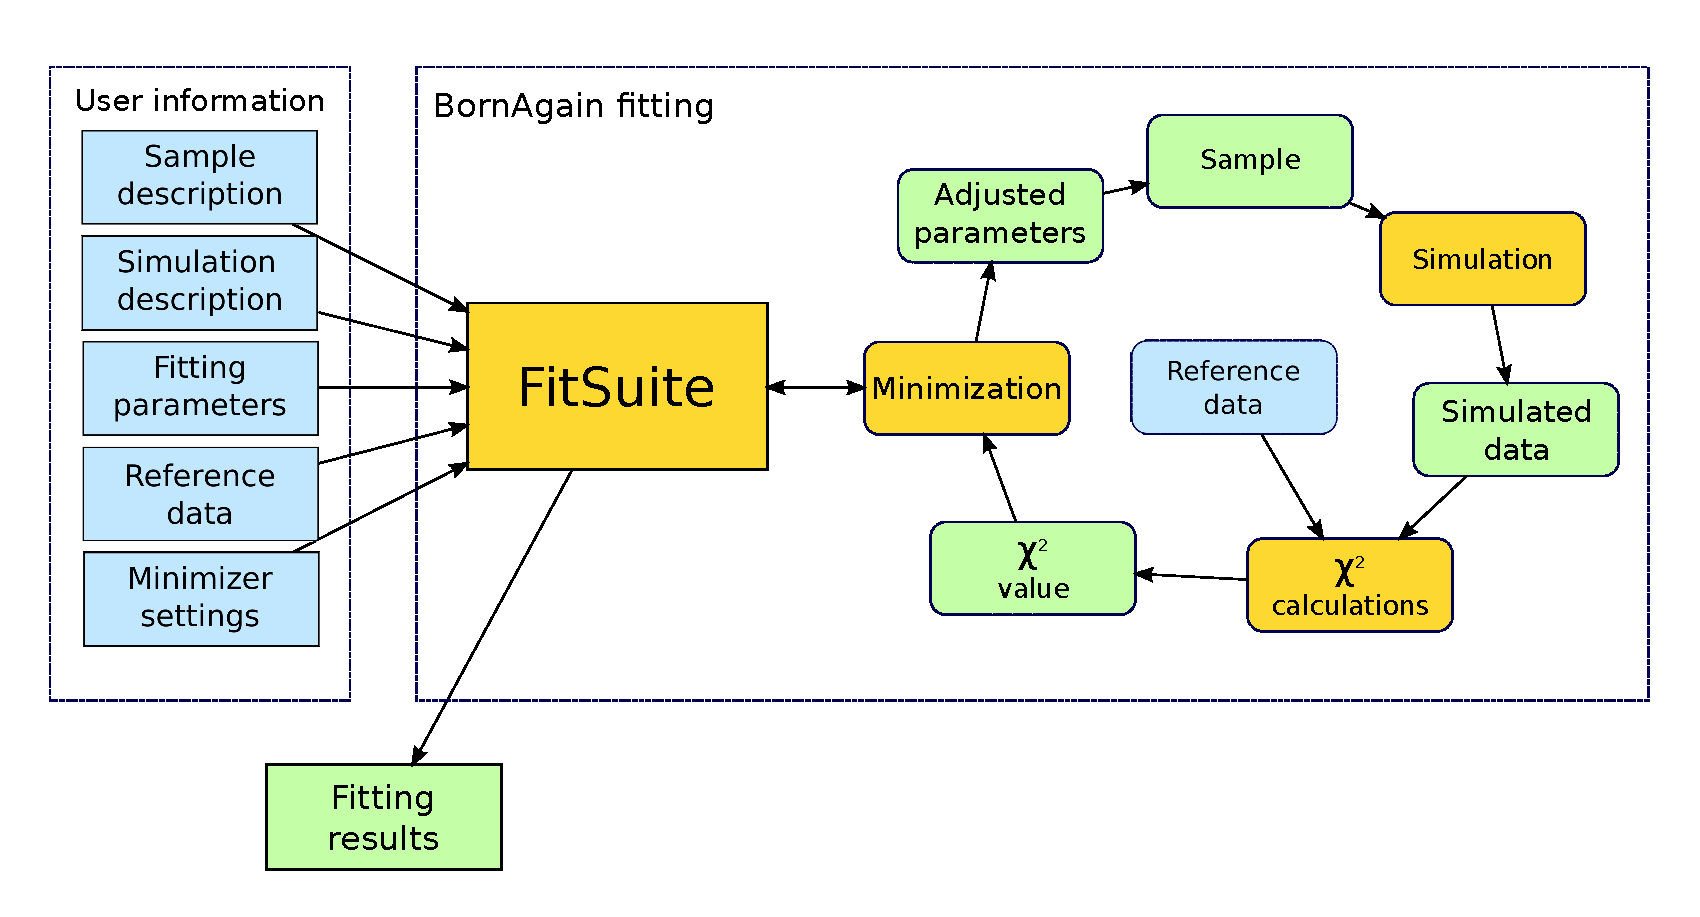
\includegraphics{Figures/minimization_workflow.eps}}
\caption{
Fitting work flow.
}
\label{fig:minimization_workflow}
\end{figure}
Before running the fitting the user is required to prepare a number of data and to
configure fitting kernel of \BornAgain\ . Necessary stages consist of

\begin{itemize}
\item Preparing sample and simulation description (multilayer, beam, detector parameters).
\item Choice of fitting parameters.
\item Loading of reference data.
\item Defining minimization settings.
\end{itemize}

The class \Code{FitSuite} contains the main functionalities to be used for the fit
and serve as main gate between user and fitting work flow. 
The later involve iterations during which

\begin{itemize}
\item The minimizer makes an assumption about optimal sample parameters.
\item These parameters are propagated to the sample.
\item The simulation is performed for the given state of the sample.
\item Simulated data (intensities) are propagated to the $\chi^2$ module.
\item The later performs calculation of $\chi^2$-value using simulated and reference data.
\item $\chi^2$-value is propagated to the minimizer which makes new assumption about optimal sample parameters.
\end{itemize}

Iteration process is going on without user intervention under the control of currently selected minimization algorithm. It stops 
\begin{itemize}
\item when the maximum number of iteration steps has been exceeded
\item when the function's minimum has been reached within the tolerance window 
\item if the minimizer could not improve the values of the parameters 
\end{itemize}

After the control is returned to the user application fitting results can be retrieved.
That consist of the best $\chi^2$ value found, corresponding optimal sample parameters and intensity map simulated with this set of parameters.

Details of \Code{FitSuite} class implementation and description
of each interface are given in \SecRef{FitSuiteClass}. The following parts of this section will detail each of
the main stages necessary to run fitting procedure.


%%%%%%%%%%%%%%%%%%%%%%%%%%%%%%%%%%%%%%%%%%%%%%%%%%%%%%%%%%%%%%%%%%%%%%%%%%%%%%%
%
%%%%%%%%%%%%%%%%%%%%%%%%%%%%%%%%%%%%%%%%%%%%%%%%%%%%%%%%%%%%%%%%%%%%%%%%%%%%%%%
\subsection{Preparing sample and simulation description.}

This step is similar for any simulation using \BornAgain\ (see \SecRef{Simulation}). It consists in first characterizing  the geometry of the system: the particles 
(shapes, sizes, refractive
indices), the different layers (thickness,
order, refractive index, a possible roughness of the interface), the
interference between the particles and the way they are distributed in
the layers (buried particles or particles sitting on top of a
layer). 
Then we specify the parameters of the input beam and of the
output detector.


%%%%%%%%%%%%%%%%%%%%%%%%%%%%%%%%%%%%%%%%%%%%%%%%%%%%%%%%%%%%%%%%%%%%%%%%%%%%%%%
%
%%%%%%%%%%%%%%%%%%%%%%%%%%%%%%%%%%%%%%%%%%%%%%%%%%%%%%%%%%%%%%%%%%%%%%%%%%%%%%%
\subsection{Choice of parameters to be fitted}
In principle, every parameter used in the construction of the sample
can be used as a fitting parameter. For example, the particles'
heights, radii or the layer's roughness or thickness could be selected using
parameter pool mechanism. 
That mechanism is explained in details in \SecRef{WorkingWithSampleParameters} and it is recommended to read it before proceeding further.

User specifies selected sample parameters as a fit parameter using \Code{FitSuite}
and its \Code{addFitParameter} method

\begin{lstlisting}[language=shell, style=commandline]
fit_suite = FitSuite()
fit_suite.addFitParameter(<name>, <value>, <AttLimits>)
\end{lstlisting}

Here the \Code{<name>} correspond to the name of the parameter in the sample's parameter pool.
By using wildcard's in the parameter name the group of sample parameters, corresponding to the given
pattern, can be associated with single fitting parameter and 
fitted simultaneously to get common optimal value.

The second parameter \Code <value> correspond to the initial value of fitting parameter
while the third one \Code{<AttLimits>} corresponds to
the boundaries imposed on the range of variations of that value. It can be
\begin{itemize}
\item \Code{limitless()} by default, 
\item \Code{fixed()}, 
\item \Code{lowerLimited(<min\_value>)}, 
\item \Code{upperLimited(<max\_value>)}, 
\item \Code{limited(<min\_value>, <max\_value>)}.
\end{itemize}
where \Code{<min\_value>} and \Code{<max\_value>} are
double values corresponding to the lower and higher boundary respectively.


%%%%%%%%%%%%%%%%%%%%%%%%%%%%%%%%%%%%%%%%%%%%%%%%%%%%%%%%%%%%%%%%%%%%%%%%%%%%%%%
%
%%%%%%%%%%%%%%%%%%%%%%%%%%%%%%%%%%%%%%%%%%%%%%%%%%%%%%%%%%%%%%%%%%%%%%%%%%%%%%%
\subsection{Associating reference and simulated data.}

The minimization procedure deals with a pair of reference data (normally
associated with experimental data) and the theoretical model (presented by the sample and the simulation descriptions).

We assume that the experimental data is a two-dimensional intensity 
matrix as function of the output scattering
angles $\alpha_f$ and $\phi_f$ (see Fig.~\ref{fig:multil3d}).
The user is required to provide the data in the form of ASCII file containing axes
binning description and the intensity data itself. 
\vspace*{2mm}

\ImportantPoint{Remark:}{
We recognize the importance of the support of most common data formats. We are going to provide
this feature in the following releases and welcome user requests on that subject.
}
\vspace*{1mm}

To associate the simulation with the reference data the method \newline
\Code{addSimulationAndRealData} has to be used as shown
\begin{lstlisting}[language=python, style=eclipseboxed,numbers=none]
fit_suite = FitSuite()
fit_suite.addSimulationAndRealData(<simulation>, <reference>, <chi2_module>)
\end{lstlisting}

here \Code{<simulation>} correspond to the \BornAgain\ simulation object with sample, beam and detector fully defined, \Code{<reference>} correspond to the experimental data object obtained from ASCII file and \Code{<chi2\_module>} is an optional parameter for advanced 
control of $\chi2$ calculations.

There is a possibility to call given method more than once to submit more than one pair of
\Code{<simulation>, <reference>} to the fitting procedure and so to provide simultaneous fit of
some combined data set.

By using the third \Code{<chi2\_module>} parameter different normalization and weights
can be applied to let the user fully control the way $\chi2$ is calculated.
This feature will be explained in \SecRef{FittingAdvanced}.


%%%%%%%%%%%%%%%%%%%%%%%%%%%%%%%%%%%%%%%%%%%%%%%%%%%%%%%%%%%%%%%%%%%%%%%%%%%%%%%
%
%%%%%%%%%%%%%%%%%%%%%%%%%%%%%%%%%%%%%%%%%%%%%%%%%%%%%%%%%%%%%%%%%%%%%%%%%%%%%%%
\subsection{Minimizer settings.}

\BornAgain\ contains a variety of minimization engines from \Code{ROOT} and \Code{GSL}
libraries. They are listed in Table~\ref{table:fit_minimizers}.
By default \Code{Minuit2} minimizer with default settings will be used and no additional
configuration needs to be done.
The remainder of this section explains some of the expert setting which can be applied to get better 
fit results.

The default minimization algorithm can be changed using 
\Code{MinimizerFactory} as shown below
\begin{lstlisting}[language=python, style=eclipseboxed,numbers=none]
fit_suite = FitSuite()
minimizer = MinimizerFactory.createMinimizer("<Minimizer name>","<algorithm>")
fit_suite.setMinimizer(minimizer)
\end{lstlisting}

where \Code{<Minimizer name>} and \Code{<algorithm>} can be chosen from the first and
second column of Table~\ref{table:fit_minimizers} respectively. 
The list of algorithms
can also be obtained using \Code{MinimizerFactory.printCatalogue()} command.


\begin{table}[h]
\centering
\begin{tabular}{@{}lll@{}}
\hline
\hline
\textbf{Minimizer name} & \textbf{Algorithm} & \textbf{Description}\\
\hline
\Code{Minuit2} \cite{MinuitURL} & \Code{Migrad} & According to
\cite{mntutorial} best minimizer for nearly all functions,\\
 & & variable-metric method with inexact line search, \\
 & & a stable metric updating scheme,\\
 & &  and checks for positive-definiteness.\\
\hline
                                       & \Code{Simplex} & simplex method of
                                       Nelder and Mead\\ 
 & & usually slower than \Code{Migrad}, \\
 &  & rather robust with respect to gross fluctuations in the\\ & &  function
 value, gives no reliable information about \\ & &  parameter errors, \\
\hline
                                       & \Code{Combined} & minimization with
                                       \Code{Migrad} \\
                                       & & but switches to Simplex if
                                       Migrad fails to converge.\\
\hline
                                       & \Code{Scan} &  not intended to
                                       minimize, just scans the
                                       function,\\
                                       & &  one parameter at a
                                       time, retains the best value
                                       after\\ &  & each scan\\
\hline
                                       & \Code{Fumili} & optimized
                                       method for least square and log
                                       likelihood\\ & &  minimizations \\
\hline
\Code{GSLMultiMin} \cite{GSLMultiMinURL} & \Code{ConjugateFR} & Fletcher-Reeves conjugate gradient
  algorithm,\\
\hline
& \Code{ConjugatePR} & Polak-Ribiere conjugate gradient algorithm,\\ 
\hline
& \Code{BFGS} & Broyden-Fletcher-Goldfarb-Shanno algorithm,\\ 
\hline
& \Code{BFGS2} & improved version of BFGS,\\ 
\hline
& \Code{SteepestDescent} & follows the downhill gradient of the function at each step\\
\hline
\Code{GSLMultiFit} \cite{GSLMultiFitURL} & & Levenberg-Marquardt
Algorithm\\
\hline
\Code{GSLSimAn} \cite{GSLSimAnURL}& & Simulated Annealing Algorithm\\ 
\hline
\hline
\end{tabular}
\caption{List of minimizers implemented in \BornAgain. }
\label{table:fit_minimizers}
\end{table}

There are several options common for every minimization algorithms, which can be changed
before minimization starts. They are handled by \Code{MinimizerOptions} class:
\begin{lstlisting}[language=python, style=eclipseboxed, numbers = none]
options = MinimizerOptions()
options.setMaxFunctionCalls(10)
FitSuite().getMinimizer().setOptions(options)
\end{lstlisting}
In given code snippet a number of ``maximum function calls'', namely a number of times the minimizer is allowed to call the simulation, is limited to the 10. The minimizer will take that number into consideration and will try to limit number of iterations by that value.

There is also a number of expert level options common for all minimizers as well
as a number of possibilities to tune individual minimization algorithms.
They will be explained in \SecRef{FittingAdvanced}.


%%%%%%%%%%%%%%%%%%%%%%%%%%%%%%%%%%%%%%%%%%%%%%%%%%%%%%%%%%%%%%%%%%%%%%%%%%%%%%%
%
%%%%%%%%%%%%%%%%%%%%%%%%%%%%%%%%%%%%%%%%%%%%%%%%%%%%%%%%%%%%%%%%%%%%%%%%%%%%%%%
\subsection{Running the fitting ant retrieving the results.}

